% Turabian Formatting for Theses and Dissertations, 2018/08/06
%
% Developed using the turabian-formatting package (2018/08/01), available through CTAN: http://www.ctan.org/pkg/turabian-formatting
%
% Additional document class formatting options:
%
% raggedright: ragged right formatting without hyphenations
% authordate: support for the author-date citation style
% endnotes: support for endnotes

% document class handles the big-picture formatting
\documentclass{turabian-thesis}

% fancyhdr does fancy headers
\usepackage{fancyhdr}

% for glossaries
\usepackage{glossaries}

\usepackage{svg}

% microtype handles microscopic improvements
\usepackage{microtype}

% graphicx handles graphics
\usepackage{graphicx}

\usepackage{soul}

% cmap makes pdfs searchable
\usepackage{cmap}

\usepackage[utf8]{inputenc}

% csquotes handles quotations
% ellipsis handles ellipses... obviously.
\usepackage{csquotes, ellipsis}

% allows half and half in tables.
\usepackage{diagbox}

% allows multiple rows
\usepackage{multirow}

% Specify paper size with geometry package
% \usepackage[pass, letterpaper]{geometry}

% For citations, use the biblatex-chicago package
\usepackage[noibid]{biblatex-chicago}
\addbibresource{backmatter/works-cited.bib}

% For fancier tables.
\usepackage{booktabs}

% For left-aligned
% \usepackage[document]{ragged2e}

% For lorem ipsum text. use \lipsum[5] to create placeholder text.
% Very handy to get an overview of how it's going to look, but also can make you feel unreasonably confident- beware!
\usepackage{lipsum}

\usepackage{xcolor}

% hyperlinks! The option [hidelinks] makes it still black i.e. not obviously a hyperlink.
\usepackage[hidelinks]{hyperref}
\hypersetup{
    colorlinks = false,
    linkbordercolor = {white},
    urlcolor = {blue}
}

\usepackage{caption} % hypcap is true by default so [hypcap=true] is optional in \usepackage[hypcap=true]{caption}

% for referencing the titles of sections
\usepackage{nameref}

% for appendices
\usepackage{appendix}

% for including pdf pages
\usepackage{pdfpages}

\usepackage{epigraph}


\newcommand{\citetemp}[1]{(#1)}

\makeglossaries{}

\newglossaryentry{score}
{
    name=score,
    description={The document that a composer creates}
}

\newglossaryentry{text}
{
    name=text,
    description={}
}

\newglossaryentry{content}
{
    name=content,
    description={The contents of the score}
}

\newglossaryentry{technique}
{
    name=technique,
    description={An action that a performer performs.}
}

\newglossaryentry{icon} 
{
    name=icon,
    description={which have a direct physical connection to the signified. Photographs are an example of icons.}
}

\newglossaryentry{index} 
{
    name=index,
    description={which show evidence of the signified. The most common example being smoke indexing fire.}
}

\newglossaryentry{symbol} 
{
    name=symbol,
    description={which have no resemblance between the signifier and the signified; their meaning must be culturally learned. Arabic numerals, the radioactive symbol, and flags are all symbols.}
}

\newglossaryentry{denotation} 
{
    name=denotation,
    description={the basic or literal meaning of the sign (i.e.\ a rose signifies the flower of the genus \emph{Rosa} of the family \emph{Rosaceae})}
}

\newglossaryentry{connotation} 
{
    name=connotation,
    description={the secondary, culturally inferred meaning; a rose might also signify passion or love, depending on the context.}
}



% Information for title page
\title{Constructing New Techniques}
% \subtitle{An Investigation in New String Techniques}
\author{Rhys Gray}
% \course{Bachelor of Music (Honours)}
% \institution{University of Tasmania}
% \department{Conservatorium of Music}
% \location{Hobart, Tasmania}
\date{\today}


% this is where the document starts. Comment out things that you don't need.
\begin{document}

% \frontmatter{}
\maketitle

% \mainmatter{}
In the context of my thesis, `Writing Wrong Right: Composing With Extended Techniques', I examine the ways in which we can remove the barriers that composers and performers face with extended techniques.
As part of the thesis, I explore the semiology of notation, and deconstruct it to establish a `cookbook' of elements, which can be used to construct new notation for techniques that adheres to the unwritten `style guide' of existing Western musical notation.
This paper is a practical example of this; in it, I use autoethnography to show my experiences constructing both a technique, and a type of notation. 
This is intended to be representative, as a technique maps an action to a symbol, while a form of notation maps a mode of interacting with an instrument to the score;
it is intended that the reader can extrapolate from my findings along with the cookbook to construct notation to suit their purposes as required.

\section{Goals}

In this paper, I examine the interfaces used to communicate music, and synthesise a working model of ways to notate techniques that can interface with traditional Western musical notation, and extend it.
The argument being put forth is that much like a language, music notation evolves naturally, with new `words' being developed when no suitable existing `word' is found.
The system which I propose is not a constructed language like Lojban or Esperanto, which take an opinionated and prescriptive approach to language. 
Rather, the method is more like compiling a list of morphemes encountered in existing works, breaking down our existing musical language into its elements so that compoundment, affixation, and other methods of constructing new `words' may occur naturally.
With this system, we will be able to establish a dictionary of existing symbols, as well as their function.
Composers that seek to notate in new and different manners will be able to take the symbols and interfaces a la carte, and construct their own, specific to their needs.

\section{Literature Review}

\subsection{Semiotics}

A brief overview of semiotics is necessary in order for any serious discussion to be had.
Semiotics, the study of signs (read: meaningful communication), was invented concurrently by Ferdinand de Saussure and Charles Sanders Peirce independent of one another.\autocite[]{saussure}
The most appreciable difference between their models was that while Saussure held that signs were made up of a signifier (the form of the sign) and signified (its meaning), Pierce's model also had an interpretant; the object that the audience interprets the signified as (since it is impossible to replicate meaning perfectly).\autocite[]{pierce}
Signifiers are then broken up into three discrete categories; 
\begin{itemize}
\item \emph{\gls{icon}}: which have a direct physical connection to the signified. Photographs are an example of icons.
\item \emph{\gls{index}}: which show evidence of the signified. The most common example being smoke indexing fire.
\item \emph{\gls{symbol}}: which have no resemblance between the signifier and the signified; their meaning must be culturally learned. Arabic numerals, the radioactive symbol, and flags are all symbols.
\end{itemize}

Finally, our signs have two channels of information.
\begin{itemize}
\item \emph{\gls{denotation}}: the basic or literal meaning of the sign (i.e.\ a picture of a rose signifies the flower of the genus \emph{Rosa} of the family \emph{Rosaceae})
\item \emph{\gls{connotation}}: the secondary, culturally inferred meaning; a rose might also signify passion or love, depending on the context.
\end{itemize}

Interpreting these signs is described as semiosis, which Philip Tagg states is `simply the process by which meaning is produced and understood.'\autocite[156]{taggMusicMeaningsModern2013}
Semiosis happens constantly; the process of converting these words into the understanding of the concept of semiosis is, in itself, semiosis. 
Pierce argues that in between the audience and the signifier, during the process of semiosis there is the interpretant, an object that the audience creates that represents the signified (because a dog cannot exist inside our heads, but merely the idea of a dog; the reality of the dog will never be fully realised inside the mind because it lacks the gestalt of the physical thing; 
it's a construct, unable to approach the truth of the dog by virtue of its limitations).\autocite[]{pierce}
Semiosis is an important step, as the interpretant which Peirce describes is unique to the audience; we construct meaning completely independently, informed by our past experiences and knowledge.\citetemp{citation needed Pierce}
Thus, the same picture of an aunt's dog may be interpreted by the aunt as being a loving pet, whereas a neighbour might interpret the image more negatively, as `the annoying dog that wakes me up at 6am'.

Looking at Western notation, we have several instances where a symbol may hold a different context depending on the interpreter's experience-- 
the same notation is used for a harmonic and a note that is meant to be played open on a French horn.\autocite[]{schuilingNotationCulturesEthnomusicology2019}
If a musician was given a piece of sheet music without any indicator of the instrument that it was written for, their experience (or lack thereof) with one of the instruments may influence how they choose to interpret the symbol.
John Fiske categorises \begin{quotation}
    denotation [as] what is photographed, connotation [as] how it is photographed
\end{quotation}.\autocite[91]{fiskeIntroductionCommunicationStudies2011}
What the composer chooses to put on the page could be argued to be denotative, while what is omitted and how the material is presented is connotative.

Semiotics is particularly applicable in web design, where intuitive `notation' is sought after to reduce the `friction', or difficulty a user has navigating a site.
We can learn many things from the research that has been done into how to use skeuomorphic design to convey an element's function.
Our goal with constructing intuitive music notation is to reduce the `friction' just like a web designer.
We can use the connotations of existing symbols to help infer how we can construct new symbols.
As an example, the line that makes up a glissandi can be either straight, or wavy, as seen in \autoref{fig:Glissando}.
\begin{figure}
    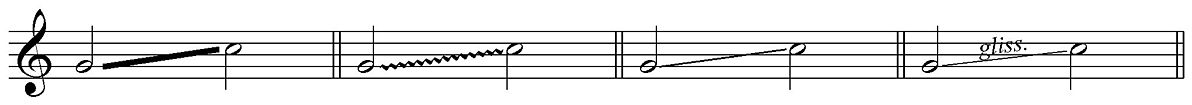
\includegraphics[]{./resources/glissando.jpg}
\caption{Various styles of glissandi}\label{fig:Glissando}
\end{figure}
The similarity of the last two examples on the right to the notation for \emph{portamento} results in a connotation with those two types being continuous, rather than having discrete pitches.
Additionally, the interpretant's instrument may also influence the meaning to them- timpanists and trombonists are more likely to interpret glissandi as continuous changes, while pianists interpret step-wise due to the nature of their instruments.\autocite[]{need to find a citation for this}
In this way, we understand that the meaning of a symbol is tied inextricably with the culture of the interpretant; attempting to make use of this cookbook for an audience not `primed' to understand it (i.e.\ one unfamiliar with Western art music conventions) is doomed to failure.
In order to produce a document that can be used reliably, the work must either be totally objective (a fool's errand in the pursuit of extracting cultural understanding of signs), or cognisant of the pitfalls and assumptions made.
To this end, the `cookbook' necessitates disclaimers specifying the assumptions made; terminology or notation used specifically in avant-garde or Renaissance music will not have any transitive qualities aiding its uptake to an audience that is not familiar with the source material.


Some symbols are not compatible with one another; a properly engraved work will never have an upbow and downbow on the same note, as the two symbols fulfill the same function.
This is what is known as a paradigmatic relationship; by virtue of the presence of one, it excludes the possibility of the other.
Looking at web design, we can draw a somewhat rough parallel to drop-down menus; there's only one slot that can be filled.
Other examples of paradigms would be the degree at which a French horn opens or mutes their instrument, which is not a binary, but a scale of `openness'.

Understanding the properties of a sign that are inherited from its history, context, and role informs what information is necessary to communicate to the reader in order for them to be able to make use of the `cookbook'.
Without a cohesive and holistic (or rather, as holistic as is possible) treatment of the signs, the intent of the `cookbook' falls short; composers must be armed with the knowledge of the context in which the sign developed, and its use in order to be able to make informed decisions.

\subsection{Argument}
In the 20th century, the `cult of the written score' developed, in which the composer prescribed more and more parameters to be interpreted literally.\autocite[]{citation very much needed}
This was in part fueled by contemporary composers being strongly opinionated in how their works should be interpreted, and partly because of the styles-- the sheer breadth of the number of parameters specified in New Complexicist works makes the interpreter pre-biased to assume that there is little room for interpretation.
This has permeated through to an underlying culture of assuming that when performing a work by a living composer that, if they wished for it to be interpreted a specific way, they would have specified that.
Unfortunately, notation is an imperfect representation of the perfect, Platonic ideal, which exists only in the mind of the composer. 
Notation is the physical manifestation of a perfect ideal, imperfectly represented as best possible by the composer.

Floris Schuiling describes music notations as \begin{quotation}
`interfaces for imagining virtual musical relations'
\end{quotation}
which is an apt description; similar meaning can be derived from verbal instructions, and the notation used is merely a vehicle through which to deliver the instructions on how to play the work.
The end result of this is that the precise vehicle through which performers obtain their instructions can be modified, mutated, and otherwise changed to better represent the imagined musical relations as the composer envisages.
This is done often when the traditional structure of Western music notation fails to account for some niche that it was not designed for; the aleatoric works of John Cage, stochastic aleatoricism of Lutoslawski, and many other 20th century composers, who sought to extend the artform to its metaphorical breaking point.
Their modifications of notation have, to varying degrees, taken root, and become accepted into the canon as valid notation; it is unlikely that the reader would have any doubt of the intended effect if presented with a Bartok pizzicato symbol above a string instrument's note.
However, these notations have been developed independent of one another, and in the current musical sphere, we are faced with an ever-increasing list of symbols to memorise, along with lengthy descriptions littering the frontmatter.

Of particular interest is the work of Ellen Fallowfield, whose thesis, `CelloMap' website and recently, application, form a comprehensive and holistic review of the ways in which a performer may `map' actions onto a cello.\autocite[]{fallowfieldCelloMapHandbook2009,fallowfieldCelloMap}
This non-opinionated and genericized method of cataloguing actions sees its contents applicable where a more specific approach would fall short, ensuring that it does not fall out of date.
In a similar way, I aim to catalogue and genericize actions from a composer's perspective, providing a suite of tools with which a composer can construct a notation to suit any imagined circumstance; be it using an animated score that changes with time, a score seen within a VR headset, or any other mode that may develop in the future.
There has been much research done into the ways that computers can interpret sheet music, an extension of OCR technology which has resulted in several market-ready tools such as PhotoScore. 
More pursuant to this study are the developments of machine-readable formats such as the GUIDO music notation system, if only as examples of the parameters that must be accounted for.

The thesis denm makes a comprehensive study of many of the strategies and reasons that performers will mark up a score with annotations. 
Additionally, it goes into discussion of the various accessibility and printing issues associated with using CYMK colour in printed scores.\autocite[22--29]{bean}
denm (Dynamic Environmental Notation of Music) is a 

Kurt Stone identifies many of the issues present in modern notation in his 1963 article in \emph{Perspectives of New Music}, and he states that \begin{quotation}
    `no other aspect of contemporary notation is more desperately in need of fundamental revision than that of rhythm.'
\end{quotation}, arguing that the existing systems of notating rhythmic ideas are either insufficient, poorly tooled, difficult to implement, or otherwise not suitable for purpose.\autocite[20--22]{stoneProblemsMethodsNotation1963}
Stone explores proportional notation as used in Stockhausen's \emph{Zeitmasse} and Cage's \emph{Music of Changes} (1951), identifying an issue where accidentals can interfere with precise placement of notes. 
This proportional notation system is very similar to the piano roll, or \emph{pianola} that is found in many Digital Audio Workstation workflows, such as Ableton, FL Studios, and Pro Tools.
The piano roll notation is arguably a superior method, as it is as literal as can be, assigning pitch to the y axis (with the label of the y axis being the matching piano key), and time to the x axis, often representing the metrical grid with lines.
However, while this workflow is suitable for DAWs, it is cumbersome to use in performance settings, and cannot be considered a genuine alternative for mapping music to an interface for performance purposes.
Stone notes this, recognising how proportional notation is ill-fitted to performer parts due to rhythmic explicitation via a `middleman' of a commonly agreed metrical unit being replaced with the much more subjective relational measurement; a crotchet is explicitly a crotchet, but a 3.3cm distance may be approximated to an imprecise element.
This can be mitigated with a common `cue' stave in parts, but as size of the ensemble grows, practicality decreases.

Stone describes notation as \begin{quotation}
    [\dots] a system of directional signs which [is] used to enable a performer conversant with them and and with the musical conventions of the era during which they were in use, to recreate a composer's \emph{artistic} vision on the basis of what the \emph{mechanical} directions implied.
\end{quotation}

He continues, stating that \begin{quotation}
    [some] of today's music is constructed in such a way that the slightest modification of \emph{any} of its measurable elements is likely to distort the inner logic of the entire work.
    In such music, only rigid sign realization is admissable; this music does not permit ``interpretation''. 
    At the same time, however, music of this nature is generally so complex that truly accurate sign realization is rarely if ever achieved in performance.
    Thus, the score and the performer have actually exchanged roles: whereas the score used to be the map designed to guide the performer towards the composer's artistic vision, it now is often completely explicit.
    On the other hand, performances are now often mere stabs in the direction of the composer's envisioned perfection of execution.
    The imprecision and variability of human performance are actually quite detrimental to the requirements of totally organized and predetermined works.\autocite[30--31]{stoneProblemsMethodsNotation1963}
\end{quotation}

This thesis aims to provide the composer with more tools to aid in the specificity of the work, so that they may more accurately and concisely communicate the desired techniques.
\section{Methodology}
\section{Case Study}

The composer and recorder player Claire Farrell approached me, asking for my opinion on how to notate an extended technique that she had been developing. 
The technique involves the recorder player covering the window hole with their index finger or hand, which results in the recorder producing a whistle like effect. 
Air pressure determines the pitch, and the degree to which the window hole is covered determines the fundamental's presence or lack thereof, with full occlusion of the window producing solely the harmonic. 

This is an ideal place in which to explore the ways in which we map actions into notation; the question becomes one of how this can be achieved in the most recognisable and orderly manner. 
Our goal of establishing a defined notation system is to ensure that it is as clear and easy to understand as possible. 

Thus began an informative exploration through the various ways that we can map sound onto an instrument. 
This is an especially interesting topic to me, as I am interested in the ways in which the semiotics of notation influence its parsing. 
We can treat this development of the notation of a new technique as a case study for best practices, and establish some ground rules on how the written form of Western art music can be adapted to accomodate new techniques that fall outside of the initial set.



% \begin{itemize}
% \item Textually, through the use of just text instructions. 
% Examples would include `mute'.
% \item Textually and pictographically, with text describing complex operations, aided by the shorthand of symbols. 
% Examples would include `mute unmute'.
% 	\item Pictographically; this would encompass all techniques that are divorced from the reality of the object, such as harmonics. 
% As this is a very broad category, it can be broken down further:
% 		\item Pictographically with symbols, such as our harmonic example.
% 		\item Pictographically, with mappings to physical objects, such as the pedal sign representing the lifting of the pedal, or the half-hole representing a partially occluded hole.
% \end{itemize}

\subsection{Building from Pre-existing Notation}

Maintaining compatibility with existing Western music notation is only possible if we follow the rules that are set out in existing symbols and structures.
This means that we cannot mutate existing symbols, or ascribe a different meaning to their common one; there are to be no uses of the piano pedal symbol to indicate a patch change on an electric keyboard.
Similarly, we cannot expect the user to intuitively understand symbols that don't follow the existing design language.

We first establish that if using a pictographic notation, that there is a point at which the instrument's window cannot be occluded any further. 
This would, logically, follow the pre-established convention of filled in black representing `more'. 
Further more, we know that there is a point at which there is no occlusion; the exact opposite. 
However, the precise point of this point is variable.

Pictographic notation is most useful when there are elements that cannot be conveyed succinctly with text; while it is true that you could notate it as `cover window with hand to produce high pitched seagull sound', it would be cumbersome to read and interpret quickly. 
Reducing that to `cover window' might result in unfortunate misinterpretations. 
Those examples also treat the act of covering the window as a binary; Claire described how the sound can change when you cover it partially, fully, or even stick your finger inside the window, blocking the free passage of air slightly to create a wholly new sound. 
So, we can safely establish that it is not feasible to use a textual direction with some degree of certainty; 
minute differences between covering the window from 30 percent to 50 percent and back to 20 percent would be unnecessarily verbose, or filled with numbers that were divorced from contextual information.

An aural equivalent can be drawn from double bass repertoire, in which a high harmonic on the bridge glissandos rapidly down to a lower partial, producing a `seagull' like effect. 
These are notated as regular harmonics, sometimes with `seagull effect' above the line. 
The double bass seagull effect is largely timbral though, and its efficacy of communicating the desired effect lies not in the notation, but in the unary nature of the intended resultant sound; a rapid dropping of a high pitch to a lower one. 
It is tied to a real world parallel, and is thus easily mapped onto the instrument.

Action parallels include the stopping of a horn with a hand, and covering windpipes on clarinets and flutes; see \autoref{fig:Asset10}. 
These are closer to the intended action, and indeed the recorder lowers a tone on full occlusion of the airway much like the horn. 
However, Claire noted an issue with the typical notation; the open circle, half-closed circle, and fully black circle had no relationship to the instrument. 
The half-occlusion of the circle was confusing as the window is a square, and fingering holes are round.
Claire was attempting to map a horn technique onto a recorder, with predictably confusing results. 

\begin{figure}
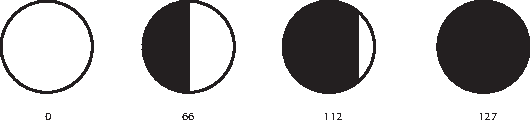
\includegraphics[width=\linewidth]{./resources/Asset 10.pdf}
\caption{Half-closed circle style}\label{fig:Asset10}
\end{figure}


I modified the notation to a rectangle, to represent the rectangular window, and added black to it to represent occlusion, moving from left to right as with the half-closed circle notation; see \autoref{fig:Asset3}.
For the sake of convenience, the level of occlusion has been mapped to a MIDI rate, of 0 being totally un-occluded, with 127 being fully occluded.

\begin{figure}
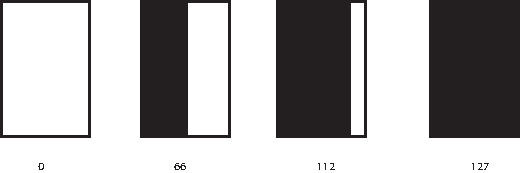
\includegraphics[width=\linewidth]{./resources/Asset 3.pdf}
\caption{Modified to a rectangle}\label{fig:Asset3}
\end{figure}

However, this was obviously inappropriate, as the action of occluding the window is not a left-to-right action.
I changed it so the black increased upwards as the notation dictated further occlusion of the window as seen in \autoref{fig:Asset1}. 
This mapped similar to how a MIDI expression level is displayed as a bar graph in DAWs. 
\begin{figure}
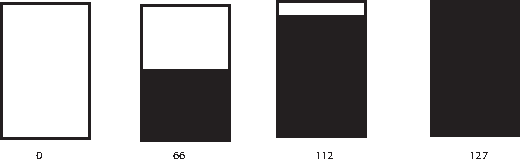
\includegraphics[width=\linewidth]{./resources/Asset 1.pdf}
\caption{MIDI style range}\label{fig:Asset1}
\end{figure}

But this too posed difficulties, as the instrument's window wasn't on the bottom of the instrument, and the hand comes \emph{down} to occlude the window. 
Rotating the image 180 degrees, I found the clearest notation yet; a picture that mapped both the intended one dimensional attribute of occlusion, as well as the action onto the instrument.

\begin{figure}
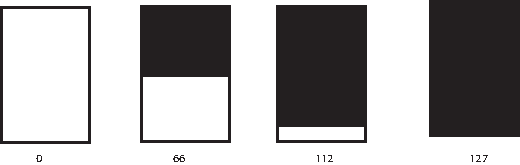
\includegraphics[width=\linewidth]{./resources/Asset 2.pdf}
\caption{Inverted MIDI style range}\label{fig:Asset2}
\end{figure}

And yet, we found there was still an outlying use-case that was not accounted for; the action of pushing the finger (or, indeed, abstracted out to any object) into the window. 
This posed an interesting issue, as it challenged our one-dimensional range attribute with needing to either accommodate the inclusion of a further attribute, or a method of delineating the cutoff point for total occlusion and where the `further in' position began. 
Further compounding the issue is the fact that there is no self-evident physical point at which further insertion is impossible; 
while the occlusion has a constant point where no further occlusion is possible (i.e.\ the window is a finite opening that can be eclipsed totally), one could theoretically put objects into the window as far as physically possible.
Further attempts were made, experimenting with a perspective representation of the window to communicate a `further in' style in the single symbol; 

\begin{figure}
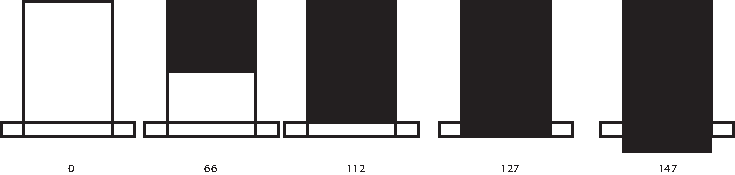
\includegraphics[width=\linewidth]{./resources/Asset 4.pdf}
\caption{First attempt; without upper limit}\label{fig:Asset4}
\end{figure}

\begin{figure}
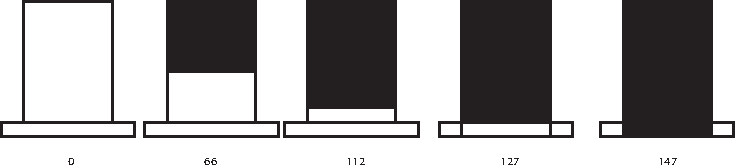
\includegraphics[width=\linewidth]{./resources/Asset 5.pdf}
\caption{Second attempt; upper limit defined}\label{fig:Asset5}
\end{figure}

\begin{figure}
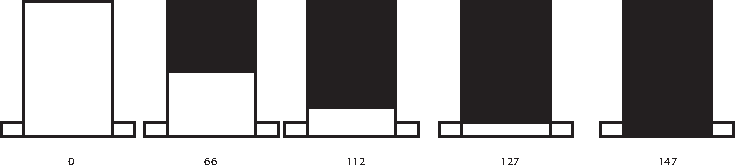
\includegraphics[width=\linewidth]{./resources/Asset 6.pdf}
\caption{`Imaginary ghost finger' single perspective}\label{fig:Asset6}
\end{figure}

\begin{figure}
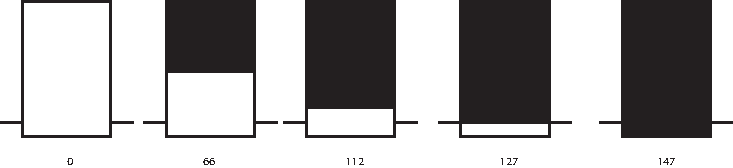
\includegraphics[width=\linewidth]{./resources/Asset 7.pdf}
\caption{Side view, upper limit defined}\label{fig:Asset7}
\end{figure}

\begin{figure}
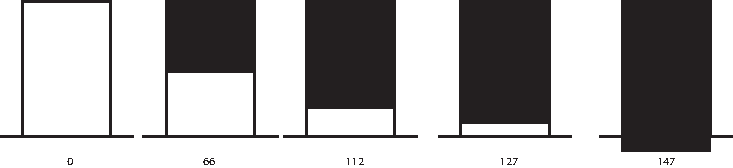
\includegraphics[width=\linewidth]{./resources/Asset 9.pdf}
\caption{Side view, without upper limit}\label{fig:Asset9}
\end{figure}

\section{Frank Zappa, Kate Soper, and Pepe Silvia}
David Dockery is a drummer that went viral years ago with his unique style of drumming in time to speech patterns of TV shows.\autocite[]{daviddockeryPepeSilviaDrums2017}
The effect is not dissimilar to that of Frank Zappa's song ``The Dangerous Kitchen'' amongst others, from his album ``The Man from Utopia''.\autocite[]{zappa}
This effect of speech being done in time with the music can also be seen in Kate Soper's work ``Only the Words Themselves Mean What They Say''.\autocite[]{soper}
Transcribing speech patterns and quantizing it to conform to a metrical grid is well established as a technique of introducing off-kilter rhythms that feel natural, however as Dockery's drumming shows, the works that are most in line with regular emotive speech contain multiple tempo and meter changes- 
showing that speech patterns are not typical iambic pentameter.

These transcriptions give us an insight into the mind of the composers, and I posit that the notated rhythms are notated thus not because the rhythms are important, but because the Western notation system does not give us adequate tools to notate speech-like cadences. 
In order to communicate the intended speech-like effect, the composers notate using the tools available, fitting their isochronous rhythms to the grid of Western notation.
This relies on either an explicit statement that the rhythms are unimportant, or the performer interpreting the subtext of the work correctly and surmising that without explicit direction.
This transcription process is lengthy, though, and when the intent is to mimic a relaxed and conversational style of speech, and not to reproduce those exact rhythms as notated, there is a degree of specificity of rhythm that is unnecessary, needlessly complicating the work.

My suggested notation is similar to non-barred music, as found in the works of Berio's Sequenzas.\autocite[]{berio}
It involves the removal of barlines, and stems of notes. 
Rhythms are derived from the lyric line underneath the stave, as depicted \hl{FINISH SENTENCE}

One of the issues with this is that it assumes both a level of flexibility in the rhythms, and a level of uniformity in how performers will interpret it; if the performer differs dramatically from the composer's rough intended idea, the work may fall out of `sync' with itself.
Mitigating this is the second version of notation, in which the beams are slightly wavy, contouring in the same manner as the \(\approx{}\) symbol. 
This reference to a pre-existing symbol for the notation of `approximately' is intended to aid comprehension by not reinventing the wheel.
This wavy-beamed notation can be used in existing Western style barred music, as well as convey a rough sense of intended rhythm when it differs from how a text would be spoken out loud.
This is useful because it gives the composer a way to `override' the performer's natural diction, without retreating back to the traditional Western notation system, which as discussed, is sometimes not suited for the notation of unfixed rhythms.

Composers that wish for a slightly more granular level of control of the rhythms can use the modified staving as notated \hl{FINISH SENTENCE}

One of the benefits of this notation system is that it maintains compatibility with the traditional Western notation system, and can be \hl{FINISH SENTENCE}

The simplest and most evident example of this technique's potential is when it is used with an instrument that can be spoken into, such as the recorder and most wind instruments. 
In the example work provided, the text is legible, but also can be used in tandem with regular notation systems, in a manner similar to that of Lutoslawski's stochastic aleatoricism.\autocite[]{lutoslawski}
Like Lutoslawski's system, there is \hl{FINISH SENTENCE}

\subsection{Speech, Rhythm, and Music}
There is a long history of where speech and music intersect, at the crossroads of rhythm. 
Many languages are tonal, and thus pitch can also play a part in the meaning of the speech. 
However, we will just be looking at how speech interacts with music within the perimeter of English, for the purposes of this article. 

Speech is naturally coded into stressed and unstressed pairs, which help define the flow. 
Using Jassem's system of rhythmic organisation, the Narrow Rhythm Unit (NRU) is described as one stressed syllable and any number of following unstressed syllables belonging to the same word.\autocite[]{hillResultsPreliminaryStudy1977}
All the other unstressed syllables which are not part of the NRU belong to the anacrusis (ANA). 

Using this system, we have a convenient way for a composer to anticipate roughly the duration of their various words; anacruses are pronounced as quickly as possible, while the NRU is isochronous, with the speaker attempting to align them with an internal grid. 
Languages that make use of syllable based timing would necessitate a different notation system, but for English texts, it makes sense to exploit its inherent stress timing. 
These stress timings can be used as a method of applying another degree of control over the interpretation of the text, where the composer is able to anticipate lexical stress with a relatively high degree of confidence, whereas the prosodic stress variabilities can be mitigated with formatting techniques that are found in regular text script.
Bold fonts, italicization, parentheses, and a host of other notational elements can be used to ensure the stress is placed in the right place. 
This notations serve both as a means of enforcing correct interpretation (``I didn't say she stole my coat'' can have any word stressed for a different meaning), and as a means of enforcing correct rhythmic placement.

Notation often seeks to emulate the cadences of speech, and there has been much research into how speech falls into a natural iambic pentameter of sorts. 
Music notation is gridded, with on-beats and off-beats, and notating rhythms which fall off the tongue easily can turn into a very complex affair, with a lot of black ink devoted to ensuring that the rhythms do not lock into the grid in predictable fashions. 
Lutoslawski uses stochastic aleatory in a somewhat similar fashion, using repetitions which do not necessarily ``lock in'' to the grid.

One of the useful aspects of this is that it augments the rhythmic channel with additional subtextual information-- a performer that is taking the rhythmic information from a text concerned with anger would conceivably perform a more emotional rendition than one in which the rhythmic information was communicated with standard staff notation.

The isochrony hypothesis states that humans innately impose a rhythmic grid onto sound in order to parse and process it, dividing it into common integers such as 2, 3, 4, 8. 
In the absence of a consensus as to the relation of isochronous beat and stress boundaries, the human internal voice can achieve a similar effect, with a greater degree of variability from person to person-- 
where there is no clear beat structure, speech is typically in iambic pentameter, and can act as a surrogate, with a high degree of stochastic variation based both on the person and their diction. 

This is distinct from Sprechstimme and recitative because the pitch content is defined, but the rhythmic content is not, and is derived from the player; 
there's some semblance of predictability with how a performer will likely perform it since there are only so many ways to say ``How kind of you to let me come'', but the precise timings will likely be different with every performer, and likely differ every time a performer plays the work. 

Recitative is similar, but pre-biases the performer towards a gridded treatment of the musical material which I posit would be less of an issue if the work had untimed notation. 

The use of the barred staff notation system predisposes a performer (typically singer) to work within the bars- granted, the performer may use rubato and fall out of sequence with the rest of the ensemble, but the end result is almost always the performer falling back in time with the ensemble. 
This is fine, but does not quite meet the goals.

Proportional notation as seen in Berio's Sequenza for Flute has its own shortcomings; the stemmed notation poses no significant benefit, and does not diverge quite cleanly from traditional notation. 
On first glance, the work can appear to simply be poorly engraved, an issue which the speech-notation system avoids.

Perhaps the most closely aligned is the system of Gregorian Chant, in which notation is achieved through neumes. 
However, the neumal system is typically reliant on a conductor guiding the performers in unison; the gridded system still exists, it is just superimposed on the music by the players.

The most useful circumstances for this form of non-timed notation, or ``Words Without Songs'' is likely in the application of poetry or monologues. 
Words with rhyming conventions are naturally predisposed to adopting a gridding, which may render the use of this non-timed notation pointless. 
Speeches, poems, and other forms of text which do not make use of iambic pentameter will therefore manifest a more distinctly different rhythmic fingerprint than rhymed lyrics. 

Using non-timed notation, we can explore exciting possibilities by imbuing our performers with a degree of independence in group contexts; 
they have the freedom to play rhythms at their own pace. 
Additionally, the addition of another information channel means that they will be able to derive further meaning from the work. 
Consider the impact of a quartet that is playing a traditional call and response type of dialogue, when they are given ``lyrics'' for their music, which will directly inform their mindset and performance. 
With the addition of words without songs, an argument between two voices is literalised, and could only benefit from the change, bringing with it an added dimension for performers to explore. \hl{FINISH ARGUMENT}
% \include{mainmatter/conclusion}

% \backmatter{}

% \begin{appendixes}
%     \include{backmatter/app0}
%     \include{backmatter/app5}
%     \include{backmatter/app1}
%     \include{backmatter/app2}
%     \include{backmatter/app3}
%     \include{backmatter/app4}
%     % \include{backmatter/appendixb}
% \end{appendixes}

% \printbibliography{}
\clearpage
\printglossary{}
\end{document}
